\documentclass[11pt,a4paper]{scrartcl}
\typearea{12}
\usepackage{graphicx}
\usepackage{pstricks}
\usepackage{listings}

\usepackage{tikz}
\usepackage{tikzscale}
\usepackage{pgfplots}

\usepackage{pgf}
\usepackage[utf8]{inputenc}
\usetikzlibrary{arrows,automata}
\usetikzlibrary{positioning}


\tikzset{
    state/.style={
           rectangle,
           rounded corners,
           draw=black, very thick,
           inner sep=2pt,
           text centered,
           },
}
\tikzset{
    on/.style={
           circle,
           draw=red, very thick,
           inner sep=2pt,
           fill=red!25,
           },
}


\tikzset{
    off/.style={
           circle,
           draw=blue, very thick,
           inner sep=2pt,
           text centered,
           },
}


\pgfplotsset{compat=1.8}


\lstset{language=python}
\pagestyle{headings}
\markright{Computational Neuroscience - 9 hippocampus}
\begin{document}

\subsection*{Introduction}
These notes are about the hippocampus.

\subsection*{Anatomy of the hippocampus}

The hippocampus is situated at the edge of the cortex and is divided
into two main areas. The hippocampus complex is distinctive in shape
and these are named for the shape
\begin{itemize}
\item Cornu Ammonis (CA) - meaning the \textsl{horn of Ammon}, an
  Egypian god of ferility with curved horns. The CA is usually divided
  into four regions, labelled CA1 through to CA4.
\item Dentate Gyrus (DG)- gyrus is the name given to the ridges in the
  cortex, dentate means \textsl{with teeth}. The dentate gyrus is one
  of the few areas of the adult brain that exhibits neurogenesis.
\end{itemize}
In addition, the main input to the hippocampus comes from the
\begin{itemize}
\item Entorhinal Cortex (EC) - entorhinal means \textsl{near the smell processing area}. 
\end{itemize}
and in this discussion this will be treated along with the hippocampus
since it partiticipates in hippocampal processing.

\begin{figure}
\begin{center}
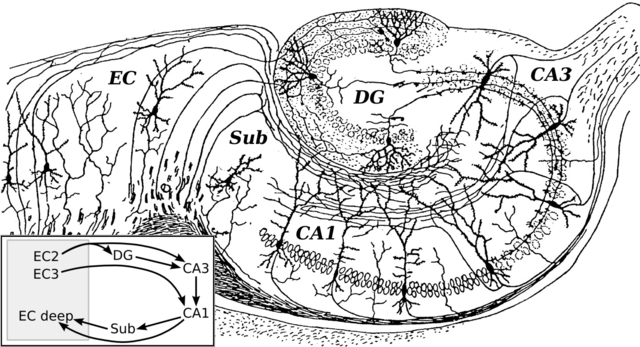
\includegraphics[width=10cm]{640px:CajalHippocampus_(modified).png}
\end{center}
\caption{The hippocampus. This is a modified image originally due to
  Cajal, probably from his 1911 book, the inset shows the approximate
  connectivity. [From
    \texttt{http://en.wikipedia.org/wiki/File:CajalHippocampus\_(modified).png}]\label{fig:hippocampus}}
\end{figure}


\begin{figure}
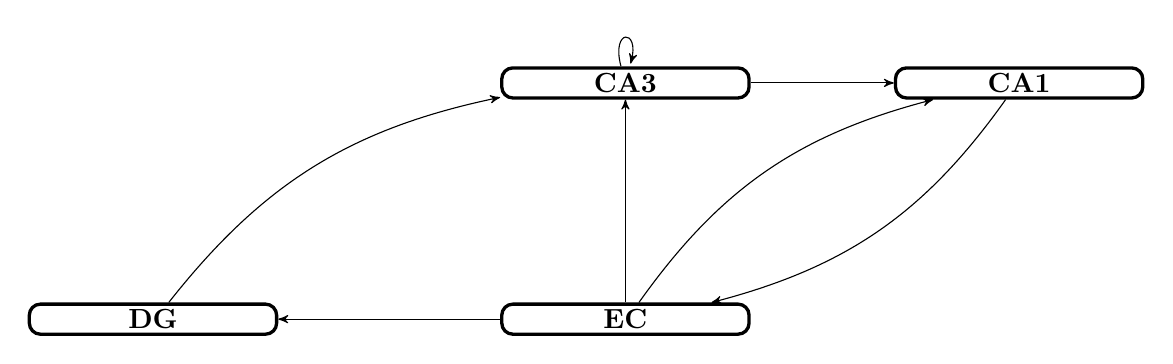
\begin{tikzpicture}[->,>=stealth']

 \node[state,text width=3cm](DG) 
 {\textbf{DG}
  };
  
 \node[state, 
 node distance=6cm,
 text width=3cm,  
 right of=DG,     
 yshift=+3cm](CA3)
 {\textbf{CA3}
 };
 
 \node[state,
  below of=CA3,
  yshift=-2cm,
  anchor=center,
  text width=3cm] (EC) 
 {\textbf{EC}
 };

 \node[state,
  right of=CA3,
  node distance=5cm,
  anchor=center,
text width=3cm] (CA1) 
 {\textbf{CA1}
 };

 \path (DG) 	edge[bend left=20]  (CA3)
       (EC)  edge (DG)
 (EC)  edge (CA3)
 (EC)  edge[bend left=20] (CA1)
 (CA1)  edge[bend left=20] (EC)
 (CA3)  edge (CA1)
 (CA3)  	edge[loop above]   (CA3)
;

\end{tikzpicture}
\caption{Connectivity of the hippocampus. A rough diagram showing the
  major connections between the areas of the connectivity. The set of
  axons running from EC to DG, CA3 and CA1 is called the perforant
  pathway, the mossy fibres run from DG to CA3 and the Schaffer
  collateral fibers go from CA3 to CA1. The loop on CA3 is supposed to
  represent the high level of recurrent connections in that
  regio.\label{fig:connectivity}}
\end{figure}

\subsection*{The role of the hippocampus}
The role of any brain region is complex and the hippocampus is no
exception. It may play a role in olefaction for example, however, it
is widely believed that its principle role is in memory and in
constructing spatial maps. Studying patients with hippocampal damage
shows that it is involved in declarative memory, that is the sort of
memory that can be described in words. It does not play a role in
procedural memory, the memory process which allows us to learn new
motor skills. It appears, again from patients with hippocampal damage,
that some long term memories are stored outside the hippocampus.

The best studied function of the hippocampus is spatial memory. There
are cells in rat CA1 known as place cells which fire in response to
specific location, an example is shown in Fig.~\ref{fig:place}. These
were first discovered in 1971 \cite{OKeefeDostrovsky1971a} and show
both that the hippocampus has a role in spatial memory and that the
memory encoding is very sparse. Another, striking, example was
discovered in 2005 in humans \cite{QuianQuirogalEtAl2005a}. Recordings
were taken from electrodes implanted for medical reasons in patients
with focal epilepsy, these patients are required as part of an
investigation into their epilepsy to spend time with the electrodes
implanted; during this time many generously agree to take part in
scientific investigations. They were shown many images while the
activity of individual cells were monitored. It was found that some
cells respond to very specific stimuli and that this stimulus can be
quite abstract. In the most quoted example a cell in hippocampus in
one patient was found which responded to pictures of Jennifer
Aniston. It did this irrespective of how she appeared, but did not
respond to other famous and non-famous faces, or curiously to pictures
of Jennifer Aniston with Brad Pitt, her spouse at that time. Again,
this demonstrates a role in memory, but one that involves very sparse
responses.

\begin{figure}
\begin{center}
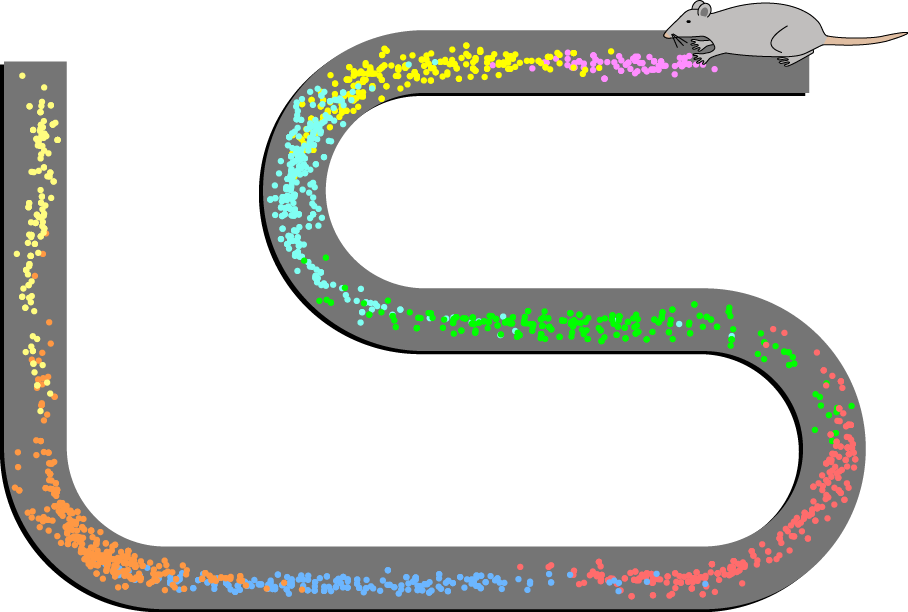
\includegraphics[width=8cm]{Place_Cell_Spiking_Activity_Example.png}
\end{center}
\caption{Place cells. This shows the firing activity of eight different cells in CA1 of a rat moving along a path, the dots correspond to spikes. [From \texttt{http://en.wikipedia.org/wiki/Place\_cell}]\label{fig:place}}
\end{figure}

\subsection*{Auto-associative memory}
The standard paradigm for memory in the hippocampus is
\textsl{auto-associative} memory. Auto-associative memories are
patterns representing memories along with some dynamics that complete
partial patters. Imagine a sequence of on-off neurons
\begin{center}

\begin{tikzpicture}
\filldraw[color=red!60, fill=red!25, very thick](0,0) circle (.25);
\filldraw[color=blue!60, fill=red!0, very thick](1,0) circle (.25);
\filldraw[color=red!60, fill=red!25, very thick](2,0) circle (.25);
\filldraw[color=blue!60, fill=red!0, very thick](3,0) circle (.25);
\filldraw[color=blue!60, fill=red!0, very thick](4,0) circle (.25);
\filldraw[color=red!60, fill=red!25, very thick](5,0) circle (.25);
\filldraw[color=blue!60, fill=red!0, very thick](6,0) circle (.25);
\filldraw[color=blue!60, fill=red!0, very thick](7,0) circle (.25);
\filldraw[color=blue!60, fill=red!0, very thick](8,0) circle (.25);
\end{tikzpicture}
\end{center}
where the filled circles correspond to on. Recall occurs when the
network is presented with a partial pattern and evolves into the
complete patterns.
\begin{center}
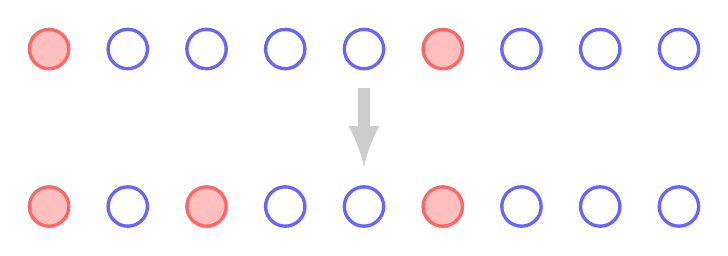
\begin{tikzpicture}
\filldraw[color=red!60, fill=red!25, very thick](0,2) circle (.25);
\filldraw[color=blue!60, fill=red!0, very thick](1,2) circle (.25);
\filldraw[color=blue!60, fill=red!0, very thick](2,2) circle (.25);
\filldraw[color=blue!60, fill=red!0, very thick](3,2) circle (.25);
\filldraw[color=blue!60, fill=red!0, very thick](4,2) circle (.25);
\filldraw[color=red!60, fill=red!25, very thick](5,2) circle (.25);
\filldraw[color=blue!60, fill=red!0, very thick](6,2) circle (.25);
\filldraw[color=blue!60, fill=red!0, very thick](7,2) circle (.25);
\filldraw[color=blue!60, fill=red!0, very thick](8,2) circle (.25);
\coordinate (a) at (4,1.5);
\coordinate (b) at (4,0.5);
\draw[->, >=latex, black!20!white, line width=4pt]   (a) to (b) ;
\filldraw[color=red!60, fill=red!25, very thick](0,0) circle (.25);
\filldraw[color=blue!60, fill=red!0, very thick](1,0) circle (.25);
\filldraw[color=red!60, fill=red!25, very thick](2,0) circle (.25);
\filldraw[color=blue!60, fill=red!0, very thick](3,0) circle (.25);
\filldraw[color=blue!60, fill=red!0, very thick](4,0) circle (.25);
\filldraw[color=red!60, fill=red!25, very thick](5,0) circle (.25);
\filldraw[color=blue!60, fill=red!0, very thick](6,0) circle (.25);
\filldraw[color=blue!60, fill=red!0, very thick](7,0) circle (.25);
\filldraw[color=blue!60, fill=red!0, very thick](8,0) circle (.25);
\end{tikzpicture}
\end{center}
The idea is that the hippocampus implements a network which performs auto-associative memory.

\subsection*{A model of CA3}
Here a highly simplified model of CA3 is presented
\cite{Amit1992a}. In this model CA3 is all-to-all connected and made
up of McCulloch-Pitts neurons \cite{McCullochPitts1943a}. We will
consider the dynamics of these neurons shortly, for now it is enough
to note that they are binary neurons with on and off states, this
would correspond, biologically, to firing and not firing and obviously
abstracts away all the details of firing along with the possibility of
there being different firing rates. We will call the on state
\lq{}1\rq{} and the off state \lq{}0\rq{}. Now let $N$ be the number
of neurons, $x_i$ the activity of neuron $i$ and $w_{ij}$ the strength
of the connection for $i$ to $j$. The sparseness, the average
proportion of neurons active at any one time is $a$, this is believed
to be very small in actual neurons. For this simple model $w_{ij}=w_{ji}$.

During learning the patterns are activated and plastic changes are
made to the synapse strength according to a simple correlation based Hebbian plasticity rule.
\begin{equation}
\Delta w_{ij}=\eta (x_i-a)(x_j-a)
\end{equation}
where $\eta$ is the learning rate, often a small number, but, in
hippocampus were memories need to be learned quickly, possibly during
a single presentation, $\eta$ is large. Since $a$ is very small too
for real networks there will be a large increase for the connection
between two neurons that are active at the same time, a tiny increase
for pairs neurons that are inactive at the same time and a medium size
decrease for pairs of neurons where one is active and one
inactive. See Fig.~\ref{fig:hebb}.

\begin{figure}
\begin{center}
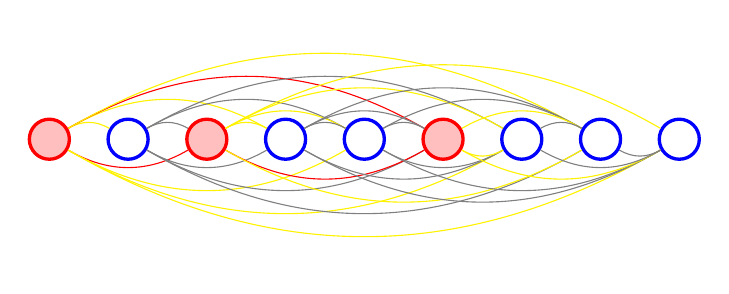
\begin{tikzpicture}
\node[on,text width=0.35cm](0){};
\node[off,text width=0.35cm,right of = 0](1){};
\node[on,text width=0.35cm,right of = 1](2){};
\node[off,text width=0.35cm,right of = 2](3){};
\node[off,text width=0.35cm,right of = 3](4){};
\node[on,text width=0.35cm,right of = 4](5){};
\node[off,text width=0.35cm,right of = 5](6){};
\node[off,text width=0.35cm,right of = 6](7){};
\node[off,text width=0.35cm,right of = 7](8){};
\path (0) edge[bend left,color=yellow] (1);
\path (0) edge[bend right,color=red] (2);
\path (0) edge[bend left,color=yellow] (3);
\path (0) edge[bend right,color=yellow] (4);
\path (0) edge[bend left,color=red] (5);
\path (0) edge[bend right,color=yellow] (6);
\path (0) edge[bend left,color=yellow] (7);
\path (0) edge[bend right,color=yellow] (8);
\path (1) edge[bend left,color=gray] (2);
\path (1) edge[bend right,color=gray] (3);
\path (1) edge[bend left,color=gray] (4);
\path (1) edge[bend right,color=gray] (5);
\path (1) edge[bend left,color=gray] (6);
\path (1) edge[bend right,color=gray] (7);
\path (2) edge[bend left,color=yellow] (3);
\path (2) edge[bend left,color=yellow] (4);
\path (2) edge[bend right,color=red] (5);
\path (2) edge[bend left,color=yellow] (6);
\path (2) edge[bend right,color=yellow] (7);
\path (2) edge[bend left,color=yellow] (8);
\path (3) edge[bend left,color=gray] (4);
\path (3) edge[bend left,color=gray] (5);
\path (3) edge[bend right,color=gray] (6);
\path (3) edge[bend left,color=gray] (7);
\path (3) edge[bend right,color=gray] (8);
\path (4) edge[bend left,color=gray] (5);
\path (4) edge[bend right,color=gray] (6);
\path (4) edge[bend left,color=gray] (7);
\path (4) edge[bend right,color=gray] (8);
\path (5) edge[bend right,color=yellow] (6);
\path (5) edge[bend left,color=yellow] (7);
\path (5) edge[bend right,color=yellow] (8);
\path (6) edge[bend left,color=gray] (7);
\path (6) edge[bend right,color=gray] (8);
\path (7) edge[bend right,color=gray] (8);
\end{tikzpicture}
\end{center}
\caption{Learning in the associate network. The pattern has been imposed and connection strengths are changed. The red links increase by $\eta(1-a)^2$ and the gray by $\eta(-a)^2$, the yellow links decrease by $\eta a(1-a)$.\label{fig:hebb}}
\end{figure}

During recall some of the neurons are held in the active state and the
rest of the network evolves according to a threshold input rule. That
means each neuron has an input given by
\begin{equation}
h_i=\sum{w_{ij}x_j}
\end{equation}
and is set in the active state if $h_i>\theta$ where $\theta$ is a
threshold which is set to different values for different networks. The idea is that after learning the pattern $\{0,2,5\}$ 
\begin{center}
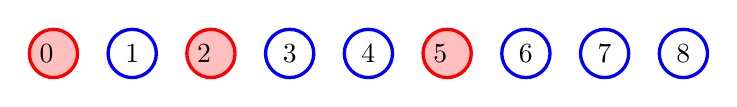
\begin{tikzpicture}
\node[on,text width=0.35cm](0){0};
\node[off,text width=0.35cm,right of = 0](1){1};
\node[on,text width=0.35cm,right of = 1](2){2};
\node[off,text width=0.35cm,right of = 2](3){3};
\node[off,text width=0.35cm,right of = 3](4){4};
\node[on,text width=0.35cm,right of = 4](5){5};
\node[off,text width=0.35cm,right of = 5](6){6};
\node[off,text width=0.35cm,right of = 6](7){7};
\node[off,text width=0.35cm,right of = 7](8){8};
\end{tikzpicture}
\end{center}
the connections between these nodes will be strong, so if the network has nodes $\{0,5\}$ activated
\begin{center}
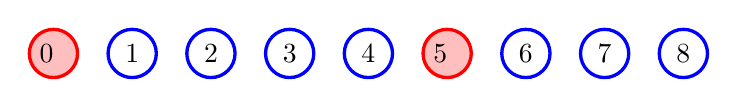
\begin{tikzpicture}
\node[on,text width=0.35cm](0){0};
\node[off,text width=0.35cm,right of = 0](1){1};
\node[off,text width=0.35cm,right of = 1](2){2};
\node[off,text width=0.35cm,right of = 2](3){3};
\node[off,text width=0.35cm,right of = 3](4){4};
\node[on,text width=0.35cm,right of = 4](5){5};
\node[off,text width=0.35cm,right of = 5](6){6};
\node[off,text width=0.35cm,right of = 6](7){7};
\node[off,text width=0.35cm,right of = 7](8){8};
\end{tikzpicture}
\end{center}
the value $h_{2}=w_{12}+w_{52}$ will be larger than threshold and the
subsequent dynamics will switch neuron 2 on. However, in this network,
if a different initial set of neurons are activated, the activity will
die away because the $h_i$ will all be sub-threshold.

\subsection*{Capacity}

When many patterns are stored it is likely that there will be
interference between them. This is illustrated in
Fig.~\ref{fig:interfere}. Although the figure shows how a single
neuron fails to participate in two patterns, for larger networks some
overlap is possible, but too much overlap prevents retrieval. In fact
the capacity is proportional to the number of neurons, $N$. A
hand-waving argument goes like this: the number of connections is
roughly $N^2$ and the amount of information in a pattern is $N$ so the
number of patterns that can be stored is $N^2/N=N$ \cite{Amit1992a}.

The capacity is also larger if there is sparseness; one way to think
of this is to observe the weight decrease between an active and
inactive connection is $\Delta w_{ij}=-\eta a (1-a)$ so the smaller
$a$ is the smaller the amount these links are decreased. Links are
decreased if, in the pattern, one neuron is active and one inactive,
they are strengthened if both neurons are active, the increase is
$\eta (1-a)^2$. Hence, it takes $1/a$ patterns where a connect is
weakened to wipe out the strengthening that results if the connect is
part of a pattern. In fact, it is estimated that the capacity of a
network is
\begin{equation}
P=\frac{k}{a}N
\end{equation}
where $k$ is constant which has been found to be about $k\approx
0.035$, this is reduced to 
\begin{equation}
P=c\frac{k}{a}N
\end{equation}
if there is missing connections, where $c$ stands for the fraction of pairs that are connected.

\begin{figure}
\begin{center}
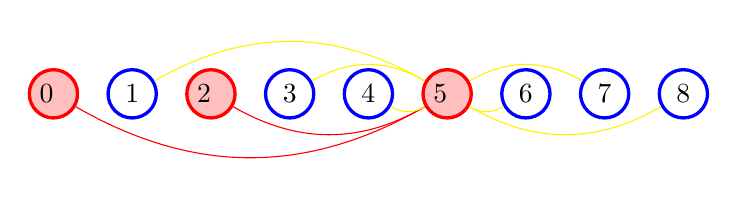
\begin{tikzpicture}
\node[on,text width=0.35cm](0){0};
\node[off,text width=0.35cm,right of = 0](1){1};
\node[on,text width=0.35cm,right of = 1](2){2};
\node[off,text width=0.35cm,right of = 2](3){3};
\node[off,text width=0.35cm,right of = 3](4){4};
\node[on,text width=0.35cm,right of = 4](5){5};
\node[off,text width=0.35cm,right of = 5](6){6};
\node[off,text width=0.35cm,right of = 6](7){7};
\node[off,text width=0.35cm,right of = 7](8){8};
\path (5) edge[bend left,color=red] (0);
\path (5) edge[bend right,color=yellow] (1);
\path (5) edge[bend left,color=red] (2);
\path (5) edge[bend right,color=yellow] (3);
\path (5) edge[bend left,color=yellow] (4);
\path (5) edge[bend right,color=yellow] (6);
\path (5) edge[bend left,color=yellow] (7);
\path (5) edge[bend right,color=yellow] (8);
\end{tikzpicture}
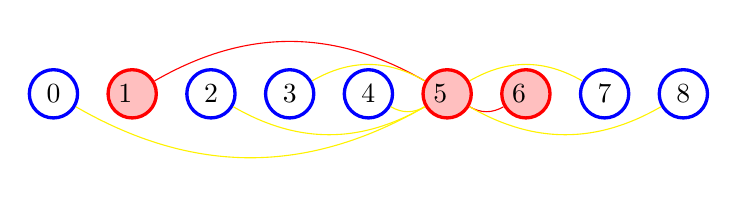
\begin{tikzpicture}
\node[off,text width=0.35cm](0){0};
\node[on,text width=0.35cm,right of = 0](1){1};
\node[off,text width=0.35cm,right of = 1](2){2};
\node[off,text width=0.35cm,right of = 2](3){3};
\node[off,text width=0.35cm,right of = 3](4){4};
\node[on,text width=0.35cm,right of = 4](5){5};
\node[on,text width=0.35cm,right of = 5](6){6};
\node[off,text width=0.35cm,right of = 6](7){7};
\node[off,text width=0.35cm,right of = 7](8){8};
\path (5) edge[bend left,color=yellow] (0);
\path (5) edge[bend right,color=red] (1);
\path (5) edge[bend left,color=yellow] (2);
\path (5) edge[bend right,color=yellow] (3);
\path (5) edge[bend left,color=yellow] (4);
\path (5) edge[bend right,color=red] (6);
\path (5) edge[bend left,color=yellow] (7);
\path (5) edge[bend right,color=yellow] (8);
\end{tikzpicture}
\end{center}
\caption{Interference in an associate network. Neuron 5 is involved in two patterns and, as a consequence, some of its connections are strengthen for one pattern and weakened for the other, if these strengthening and weakening effects are similar in size it makes it unlikely that either pattern will be accurately retrieved.\label{fig:interfere}}
\end{figure}

The actual sparseness of the brain needs to balance this advantage,
the increased capacity, along with a metabolic advantage and more
abstract computational advantage which says that a sparse coding for
information involves object recognition or segmentation against the
disadvantages, most obviously the vulnerability of the pattern to the
loss of neurons or connections and, perhaps more importantly, a sparse
code involves fewer elements and so may be less useful for
retrieval. It is hard to actually estimate sparseness in practice
since neurons are not, in reality, on-off units. A figure of $a=0.025$
is given in \cite{OReillyMunakata2000a} but, most importantly, the
hippocampus seems to sparser than other parts of the brain.

\subsection*{Correlated patterns}

The estimates above assume that the patterns are all independent. If
they aren't the capacity is reduced. If patterns share some fragments
or subpatterns then the connections in these subpatterns become very
strong, perhaps dominating other elements in the patterns, the
elements that make them different. Consider the four patterns
\begin{center}
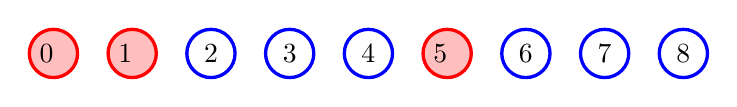
\begin{tikzpicture}
\node[on,text width=0.35cm](0){0};
\node[on,text width=0.35cm,right of = 0](1){1};
\node[off,text width=0.35cm,right of = 1](2){2};
\node[off,text width=0.35cm,right of = 2](3){3};
\node[off,text width=0.35cm,right of = 3](4){4};
\node[on,text width=0.35cm,right of = 4](5){5};
\node[off,text width=0.35cm,right of = 5](6){6};
\node[off,text width=0.35cm,right of = 6](7){7};
\node[off,text width=0.35cm,right of = 7](8){8};
\end{tikzpicture}
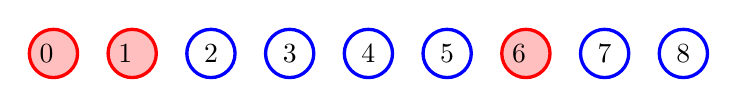
\begin{tikzpicture}
\node[on,text width=0.35cm](0){0};
\node[on,text width=0.35cm,right of = 0](1){1};
\node[off,text width=0.35cm,right of = 1](2){2};
\node[off,text width=0.35cm,right of = 2](3){3};
\node[off,text width=0.35cm,right of = 3](4){4};
\node[off,text width=0.35cm,right of = 4](5){5};
\node[on,text width=0.35cm,right of = 5](6){6};
\node[off,text width=0.35cm,right of = 6](7){7};
\node[off,text width=0.35cm,right of = 7](8){8};
\end{tikzpicture}
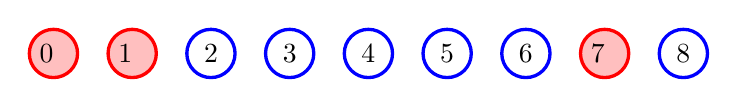
\begin{tikzpicture}
\node[on,text width=0.35cm](0){0};
\node[on,text width=0.35cm,right of = 0](1){1};
\node[off,text width=0.35cm,right of = 1](2){2};
\node[off,text width=0.35cm,right of = 2](3){3};
\node[off,text width=0.35cm,right of = 3](4){4};
\node[off,text width=0.35cm,right of = 4](5){5};
\node[off,text width=0.35cm,right of = 5](6){6};
\node[on,text width=0.35cm,right of = 6](7){7};
\node[off,text width=0.35cm,right of = 7](8){8};
\end{tikzpicture}
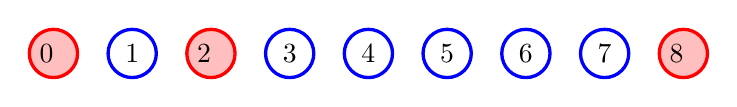
\begin{tikzpicture}
\node[on,text width=0.35cm](0){0};
\node[off,text width=0.35cm,right of = 0](1){1};
\node[on,text width=0.35cm,right of = 1](2){2};
\node[off,text width=0.35cm,right of = 2](3){3};
\node[off,text width=0.35cm,right of = 3](4){4};
\node[off,text width=0.35cm,right of = 4](5){5};
\node[off,text width=0.35cm,right of = 5](6){6};
\node[off,text width=0.35cm,right of = 6](7){7};
\node[on,text width=0.35cm,right of = 7](8){8};
\end{tikzpicture}
\end{center}
The connection between neurons 0 and 1 will become very strong because
this connection is present in three patterns out of four. It is likely
that this will result in this erroneous completion
\begin{center}
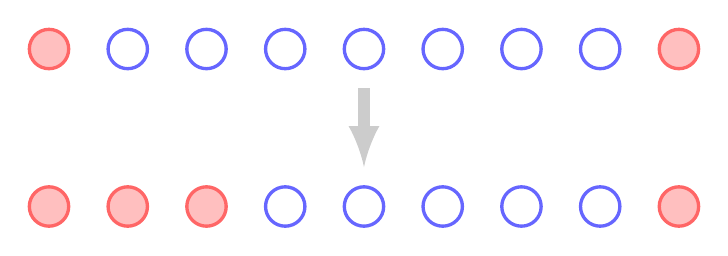
\begin{tikzpicture}
\filldraw[color=red!60, fill=red!25, very thick](0,2) circle (.25);
\filldraw[color=blue!60, fill=red!0, very thick](1,2) circle (.25);
\filldraw[color=blue!60, fill=red!0, very thick](2,2) circle (.25);
\filldraw[color=blue!60, fill=red!0, very thick](3,2) circle (.25);
\filldraw[color=blue!60, fill=red!0, very thick](4,2) circle (.25);
\filldraw[color=blue!60, fill=red!0, very thick](5,2) circle (.25);
\filldraw[color=blue!60, fill=red!0, very thick](6,2) circle (.25);
\filldraw[color=blue!60, fill=red!0, very thick](7,2) circle (.25);
\filldraw[color=red!60, fill=red!25, very thick](8,2) circle (.25);
\coordinate (a) at (4,1.5);
\coordinate (b) at (4,0.5);
\draw[->, >=latex, black!20!white, line width=4pt]   (a) to (b) ;
\filldraw[color=red!60, fill=red!25, very thick](0,0) circle (.25);
\filldraw[color=red!60, fill=red!25, very thick](1,0) circle (.25);
\filldraw[color=red!60, fill=red!25, very thick](2,0) circle (.25);
\filldraw[color=blue!60, fill=red!0, very thick](3,0) circle (.25);
\filldraw[color=blue!60, fill=red!0, very thick](4,0) circle (.25);
\filldraw[color=blue!60, fill=red!0, very thick](5,0) circle (.25);
\filldraw[color=blue!60, fill=red!0, very thick](6,0) circle (.25);
\filldraw[color=blue!60, fill=red!0, very thick](7,0) circle (.25);
\filldraw[color=red!60, fill=red!25, very thick](8,0) circle (.25);
\end{tikzpicture}
\end{center}
or even
\begin{center}
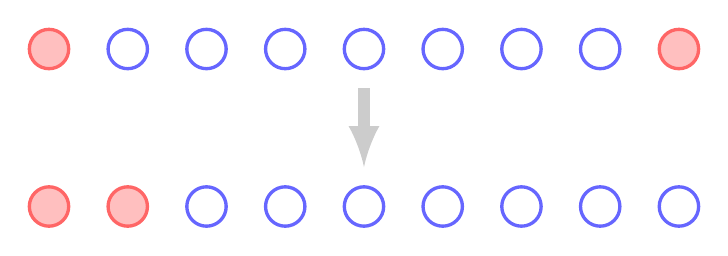
\begin{tikzpicture}
\filldraw[color=red!60, fill=red!25, very thick](0,2) circle (.25);
\filldraw[color=blue!60, fill=red!0, very thick](1,2) circle (.25);
\filldraw[color=blue!60, fill=red!0, very thick](2,2) circle (.25);
\filldraw[color=blue!60, fill=red!0, very thick](3,2) circle (.25);
\filldraw[color=blue!60, fill=red!0, very thick](4,2) circle (.25);
\filldraw[color=blue!60, fill=red!0, very thick](5,2) circle (.25);
\filldraw[color=blue!60, fill=red!0, very thick](6,2) circle (.25);
\filldraw[color=blue!60, fill=red!0, very thick](7,2) circle (.25);
\filldraw[color=red!60, fill=red!25, very thick](8,2) circle (.25);
\coordinate (a) at (4,1.5);
\coordinate (b) at (4,0.5);
\draw[->, >=latex, black!20!white, line width=4pt]   (a) to (b) ;
\filldraw[color=red!60, fill=red!25, very thick](0,0) circle (.25);
\filldraw[color=red!60, fill=red!25, very thick](1,0) circle (.25);
\filldraw[color=blue!60, fill=red!0, very thick](2,0) circle (.25);
\filldraw[color=blue!60, fill=red!0, very thick](3,0) circle (.25);
\filldraw[color=blue!60, fill=red!0, very thick](4,0) circle (.25);
\filldraw[color=blue!60, fill=red!0, very thick](5,0) circle (.25);
\filldraw[color=blue!60, fill=red!0, very thick](6,0) circle (.25);
\filldraw[color=blue!60, fill=red!0, very thick](7,0) circle (.25);
\filldraw[color=blue!60, fill=red!0, very thick](8,0) circle (.25);
\end{tikzpicture}
\end{center}
This means that auto-associative networks are not able to effectively
store anything except random patterns! This is why they have never
proved useful for machine learning; we will see later, when looking at cortical memory, that if there are multiple presentations, the memory system would have the opportunity to learn different, similar, memories. The goal here, however, is to learn the memory quickly after a small number of presentations.

In the case of hippocampus it has been proposed,
\cite{OReillyMcClelland1994a}, that this problem is solved through the
EC-DG-CA3 pathway and that the role of the dentate gyrus is to
randomize the connectivity between EC and CA3. In short, during
learning neurons in EC and CA3 are matched via DG and that the
connections from EC to DG and from DG to EC are essentially
random. This reduces overlap through a $k$-winner takes all
mechanism. Roughly, this supposed that local inhibition ensures that
the $k$ most active neurons in the DG layer \lq{}win\rq and supress
the activity of the other neurons \cite{OReillyMcClelland1994a}. The
way this might reduce overlap is shown in this cartoon where $k=1$ and
two similar patters result in a different neuron being active:
\begin{center}
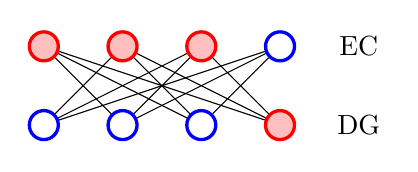
\begin{tikzpicture}
\node[on, text width=0.2cm](EC0){};
\node[on, text width=0.2cm, right of =EC0](EC1){};
\node[on, text width=0.2cm, right of =EC1](EC2){};
\node[off, text width=0.2cm, right of =EC2](EC3){};
\node[right of =EC3](EC){EC};
\node[off, text width=0.2cm, below of =EC0](DG0){};
\node[off, text width=0.2cm,right of = DG0](DG1){};
\node[off, text width=0.2cm,right of = DG1](DG2){};
\node[on, text width=0.2cm,right of =DG2](DG3){};
\node[right of =DG3](DG){DG};
\path (EC0) edge (DG1);
\path (EC0) edge (DG2);
\path (EC0) edge (DG3);
\path (EC1) edge (DG0);
\path (EC1) edge (DG2);
\path (EC1) edge (DG3);
\path (EC2) edge (DG1);
\path (EC2) edge (DG0);
\path (EC2) edge (DG3);
\path (EC3) edge (DG1);
\path (EC3) edge (DG2);
\path (EC3) edge (DG0);
\end{tikzpicture}
\end{center}
versus
\begin{center}
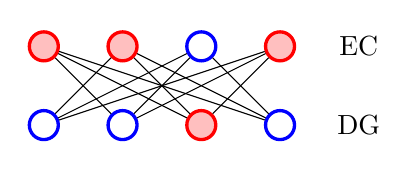
\begin{tikzpicture}
\node[on, text width=0.2cm](EC0){};
\node[on, text width=0.2cm, right of =EC0](EC1){};
\node[off, text width=0.2cm, right of =EC1](EC2){};
\node[on, text width=0.2cm, right of =EC2](EC3){};
\node[right of =EC3](EC){EC};
\node[off, text width=0.2cm, below of =EC0](DG0){};
\node[off, text width=0.2cm,right of = DG0](DG1){};
\node[on, text width=0.2cm,right of = DG1](DG2){};
\node[off, text width=0.2cm,right of =DG2](DG3){};
\node[right of =DG3](DG){DG};
\path (EC0) edge (DG1);
\path (EC0) edge (DG2);
\path (EC0) edge (DG3);
\path (EC1) edge (DG0);
\path (EC1) edge (DG2);
\path (EC1) edge (DG3);
\path (EC2) edge (DG1);
\path (EC2) edge (DG0);
\path (EC2) edge (DG3);
\path (EC3) edge (DG1);
\path (EC3) edge (DG2);
\path (EC3) edge (DG0);
\end{tikzpicture}
\end{center}
with the idea being that this randomization might be repeated in the
subsequent connection between DG and CA3. This mechanism may explain
why neurons in DG are being born all the time, perhaps their role is
to create these random connections.

\subsection*{Models of the whole hippocampus}

We are now almost in a position to consider models of the hippocampus
as a whole; so far CA1 hasn't been mentioned. It has been suggested
that the role of CA1 is to relay patterns back to EC. In learning, according to the standard model, a pattern is presented by EC:
\begin{center}
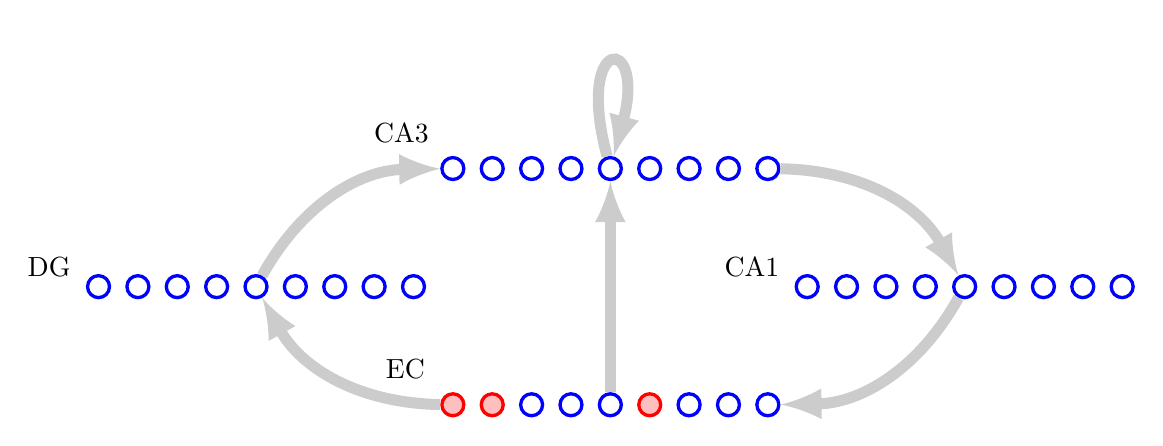
\begin{tikzpicture}
\node[on,text width=0.1cm](EC0){};
\node[on,text width=0.1cm,right of = EC0,xshift = -0.5cm](EC1){};
\node[off,text width=0.1cm,right of = EC1,xshift = -0.5cm](EC2){};
\node[off,text width=0.1cm,right of = EC2,xshift = -0.5cm](EC3){};
\node[off,text width=0.1cm,right of = EC3,xshift = -0.5cm](EC4){};
\node[on,text width=0.1cm,right of = EC4,xshift = -0.5cm](EC5){};
\node[off,text width=0.1cm,right of = EC5,xshift = -0.5cm](EC6){};
\node[off,text width=0.1cm,right of = EC6,xshift = -0.5cm](EC7){};
\node[off,text width=0.1cm,right of = EC7,xshift = -0.5cm](EC8){};

\node[off,text width=0.1cm, left of =EC0, xshift=-3.5cm,yshift=1.5cm](DG0){};
\node[off,text width=0.1cm,right of = DG0,xshift = -0.5cm](DG1){};
\node[off,text width=0.1cm,right of = DG1,xshift = -0.5cm](DG2){};
\node[off,text width=0.1cm,right of = DG2,xshift = -0.5cm](DG3){};
\node[off,text width=0.1cm,right of = DG3,xshift = -0.5cm](DG4){};
\node[off,text width=0.1cm,right of = DG4,xshift = -0.5cm](DG5){};
\node[off,text width=0.1cm,right of = DG5,xshift = -0.5cm](DG6){};
\node[off,text width=0.1cm,right of = DG6,xshift = -0.5cm](DG7){};
\node[off,text width=0.1cm,right of = DG7,xshift = -0.5cm](DG8){};

\node[off,text width=0.1cm, right of =EC8, xshift=-.5cm,yshift=1.5cm](CA10){};
\node[off,text width=0.1cm,right of = CA10,xshift = -0.5cm](CA11){};
\node[off,text width=0.1cm,right of = CA11,xshift = -0.5cm](CA12){};
\node[off,text width=0.1cm,right of = CA12,xshift = -0.5cm](CA13){};
\node[off,text width=0.1cm,right of = CA13,xshift = -0.5cm](CA14){};
\node[off,text width=0.1cm,right of = CA14,xshift = -0.5cm](CA15){};
\node[off,text width=0.1cm,right of = CA15,xshift = -0.5cm](CA16){};
\node[off,text width=0.1cm,right of = CA16,xshift = -0.5cm](CA17){};
\node[off,text width=0.1cm,right of = CA17,xshift = -0.5cm](CA18){};

\node[off,text width=0.1cm, above of =EC0,yshift=2cm](CA30){};
\node[off,text width=0.1cm,right of = CA30,xshift = -0.5cm](CA31){};
\node[off,text width=0.1cm,right of = CA31,xshift = -0.5cm](CA32){};
\node[off,text width=0.1cm,right of = CA32,xshift = -0.5cm](CA33){};
\node[off,text width=0.1cm,right of = CA33,xshift = -0.5cm](CA34){};
\node[off,text width=0.1cm,right of = CA34,xshift = -0.5cm](CA35){};
\node[off,text width=0.1cm,right of = CA35,xshift = -0.5cm](CA36){};
\node[off,text width=0.1cm,right of = CA36,xshift = -0.5cm](CA37){};
\node[off,text width=0.1cm,right of = CA37,xshift = -0.5cm](CA38){};

\draw[->, >=latex, black!20!white, line width=4pt]   (EC4) to (CA34) ;
\draw[->, >=latex, black!20!white, line width=4pt, bend left]   (EC0) to (DG4) ;
\draw[->, >=latex, black!20!white, line width=4pt, bend left]   (DG4) to (CA30) ;
\draw[->, >=latex, black!20!white, line width=4pt, bend left]   (CA38) to (CA14) ;
\draw[->, >=latex, black!20!white, line width=4pt, bend left]   (CA14) to (EC8) ;
\draw[->, >=latex, black!20!white, line width=4pt, loop above, looseness=50]   (CA34) to (CA34) ;
\node[inner sep=0,anchor=east,text width=3.3cm, left of = DG0, xshift=1.75cm,yshift=0.25cm] (DGlabel) {DG};
\node[inner sep=0,anchor=east,text width=3.3cm, left of = CA10, xshift=1.6cm,yshift=0.25cm] (DGlabel) {CA1};
\node[inner sep=0,anchor=east,text width=3.3cm, left of = CA30, xshift=1.65cm,yshift=0.45cm] (DGlabel) {CA3};
\node[inner sep=0,anchor=east,text width=3.3cm, left of = EC0, xshift=1.8cm,yshift=0.45cm] (DGlabel) {EC};
\end{tikzpicture}
\end{center}
Connections, possibily random, between EC and DG and between DG and
CA3, along with the \lq{}$k$-winner takes all\rq{} mechanism, causes activity in CA3.
\begin{center}
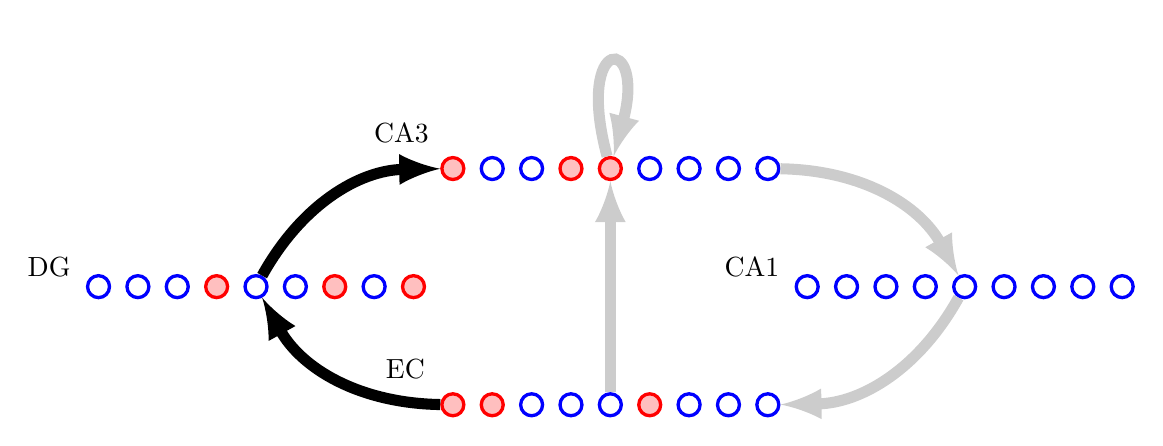
\begin{tikzpicture}
\node[on,text width=0.1cm](EC0){};
\node[on,text width=0.1cm,right of = EC0,xshift = -0.5cm](EC1){};
\node[off,text width=0.1cm,right of = EC1,xshift = -0.5cm](EC2){};
\node[off,text width=0.1cm,right of = EC2,xshift = -0.5cm](EC3){};
\node[off,text width=0.1cm,right of = EC3,xshift = -0.5cm](EC4){};
\node[on,text width=0.1cm,right of = EC4,xshift = -0.5cm](EC5){};
\node[off,text width=0.1cm,right of = EC5,xshift = -0.5cm](EC6){};
\node[off,text width=0.1cm,right of = EC6,xshift = -0.5cm](EC7){};
\node[off,text width=0.1cm,right of = EC7,xshift = -0.5cm](EC8){};

\node[off,text width=0.1cm, left of =EC0, xshift=-3.5cm,yshift=1.5cm](DG0){};
\node[off,text width=0.1cm,right of = DG0,xshift = -0.5cm](DG1){};
\node[off,text width=0.1cm,right of = DG1,xshift = -0.5cm](DG2){};
\node[on,text width=0.1cm,right of = DG2,xshift = -0.5cm](DG3){};
\node[off,text width=0.1cm,right of = DG3,xshift = -0.5cm](DG4){};
\node[off,text width=0.1cm,right of = DG4,xshift = -0.5cm](DG5){};
\node[on,text width=0.1cm,right of = DG5,xshift = -0.5cm](DG6){};
\node[off,text width=0.1cm,right of = DG6,xshift = -0.5cm](DG7){};
\node[on,text width=0.1cm,right of = DG7,xshift = -0.5cm](DG8){};

\node[off,text width=0.1cm, right of =EC8, xshift=-.5cm,yshift=1.5cm](CA10){};
\node[off,text width=0.1cm,right of = CA10,xshift = -0.5cm](CA11){};
\node[off,text width=0.1cm,right of = CA11,xshift = -0.5cm](CA12){};
\node[off,text width=0.1cm,right of = CA12,xshift = -0.5cm](CA13){};
\node[off,text width=0.1cm,right of = CA13,xshift = -0.5cm](CA14){};
\node[off,text width=0.1cm,right of = CA14,xshift = -0.5cm](CA15){};
\node[off,text width=0.1cm,right of = CA15,xshift = -0.5cm](CA16){};
\node[off,text width=0.1cm,right of = CA16,xshift = -0.5cm](CA17){};
\node[off,text width=0.1cm,right of = CA17,xshift = -0.5cm](CA18){};

\node[on,text width=0.1cm, above of =EC0,yshift=2cm](CA30){};
\node[off,text width=0.1cm,right of = CA30,xshift = -0.5cm](CA31){};
\node[off,text width=0.1cm,right of = CA31,xshift = -0.5cm](CA32){};
\node[on,text width=0.1cm,right of = CA32,xshift = -0.5cm](CA33){};
\node[on,text width=0.1cm,right of = CA33,xshift = -0.5cm](CA34){};
\node[off,text width=0.1cm,right of = CA34,xshift = -0.5cm](CA35){};
\node[off,text width=0.1cm,right of = CA35,xshift = -0.5cm](CA36){};
\node[off,text width=0.1cm,right of = CA36,xshift = -0.5cm](CA37){};
\node[off,text width=0.1cm,right of = CA37,xshift = -0.5cm](CA38){};

\draw[->, >=latex, black!20!white, line width=4pt]   (EC4) to (CA34) ;
\draw[->, >=latex, black, line width=4pt, bend left]   (EC0) to (DG4) ;
\draw[->, >=latex, black, line width=4pt, bend left]   (DG4) to (CA30) ;
\draw[->, >=latex, black!20!white, line width=4pt, bend left]   (CA38) to (CA14) ;
\draw[->, >=latex, black!20!white, line width=4pt, bend left]   (CA14) to (EC8) ;
\draw[->, >=latex, black!20!white, line width=4pt, loop above, looseness=50]   (CA34) to (CA34) ;
\node[inner sep=0,anchor=east,text width=3.3cm, left of = DG0, xshift=1.75cm,yshift=0.25cm] (DGlabel) {DG};
\node[inner sep=0,anchor=east,text width=3.3cm, left of = CA10, xshift=1.6cm,yshift=0.25cm] (DGlabel) {CA1};
\node[inner sep=0,anchor=east,text width=3.3cm, left of = CA30, xshift=1.65cm,yshift=0.45cm] (DGlabel) {CA3};
\node[inner sep=0,anchor=east,text width=3.3cm, left of = EC0, xshift=1.8cm,yshift=0.45cm] (DGlabel) {EC};
\end{tikzpicture}
\end{center}
This representation is then learned by Hebbian plasticity between EC and CA3.
\begin{center}
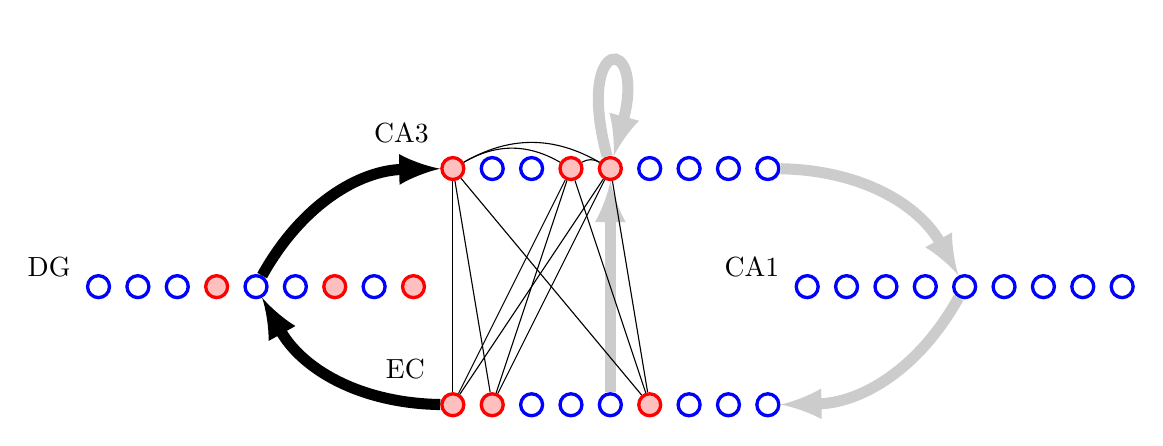
\begin{tikzpicture}
\node[on,text width=0.1cm](EC0){};
\node[on,text width=0.1cm,right of = EC0,xshift = -0.5cm](EC1){};
\node[off,text width=0.1cm,right of = EC1,xshift = -0.5cm](EC2){};
\node[off,text width=0.1cm,right of = EC2,xshift = -0.5cm](EC3){};
\node[off,text width=0.1cm,right of = EC3,xshift = -0.5cm](EC4){};
\node[on,text width=0.1cm,right of = EC4,xshift = -0.5cm](EC5){};
\node[off,text width=0.1cm,right of = EC5,xshift = -0.5cm](EC6){};
\node[off,text width=0.1cm,right of = EC6,xshift = -0.5cm](EC7){};
\node[off,text width=0.1cm,right of = EC7,xshift = -0.5cm](EC8){};

\node[off,text width=0.1cm, left of =EC0, xshift=-3.5cm,yshift=1.5cm](DG0){};
\node[off,text width=0.1cm,right of = DG0,xshift = -0.5cm](DG1){};
\node[off,text width=0.1cm,right of = DG1,xshift = -0.5cm](DG2){};
\node[on,text width=0.1cm,right of = DG2,xshift = -0.5cm](DG3){};
\node[off,text width=0.1cm,right of = DG3,xshift = -0.5cm](DG4){};
\node[off,text width=0.1cm,right of = DG4,xshift = -0.5cm](DG5){};
\node[on,text width=0.1cm,right of = DG5,xshift = -0.5cm](DG6){};
\node[off,text width=0.1cm,right of = DG6,xshift = -0.5cm](DG7){};
\node[on,text width=0.1cm,right of = DG7,xshift = -0.5cm](DG8){};

\node[off,text width=0.1cm, right of =EC8, xshift=-.5cm,yshift=1.5cm](CA10){};
\node[off,text width=0.1cm,right of = CA10,xshift = -0.5cm](CA11){};
\node[off,text width=0.1cm,right of = CA11,xshift = -0.5cm](CA12){};
\node[off,text width=0.1cm,right of = CA12,xshift = -0.5cm](CA13){};
\node[off,text width=0.1cm,right of = CA13,xshift = -0.5cm](CA14){};
\node[off,text width=0.1cm,right of = CA14,xshift = -0.5cm](CA15){};
\node[off,text width=0.1cm,right of = CA15,xshift = -0.5cm](CA16){};
\node[off,text width=0.1cm,right of = CA16,xshift = -0.5cm](CA17){};
\node[off,text width=0.1cm,right of = CA17,xshift = -0.5cm](CA18){};

\node[on,text width=0.1cm, above of =EC0,yshift=2cm](CA30){};
\node[off,text width=0.1cm,right of = CA30,xshift = -0.5cm](CA31){};
\node[off,text width=0.1cm,right of = CA31,xshift = -0.5cm](CA32){};
\node[on,text width=0.1cm,right of = CA32,xshift = -0.5cm](CA33){};
\node[on,text width=0.1cm,right of = CA33,xshift = -0.5cm](CA34){};
\node[off,text width=0.1cm,right of = CA34,xshift = -0.5cm](CA35){};
\node[off,text width=0.1cm,right of = CA35,xshift = -0.5cm](CA36){};
\node[off,text width=0.1cm,right of = CA36,xshift = -0.5cm](CA37){};
\node[off,text width=0.1cm,right of = CA37,xshift = -0.5cm](CA38){};

\draw[->, >=latex, black!20!white, line width=4pt]   (EC4) to (CA34) ;
\draw[->, >=latex, black, line width=4pt, bend left]   (EC0) to (DG4) ;
\draw[->, >=latex, black, line width=4pt, bend left]   (DG4) to (CA30) ;
\draw[->, >=latex, black!20!white, line width=4pt, bend left]   (CA38) to (CA14) ;
\draw[->, >=latex, black!20!white, line width=4pt, bend left]   (CA14) to (EC8) ;
\draw[->, >=latex, black!20!white, line width=4pt, loop above, looseness=50]   (CA34) to (CA34) ;
\node[inner sep=0,anchor=east,text width=3.3cm, left of = DG0, xshift=1.75cm,yshift=0.25cm] (DGlabel) {DG};
\node[inner sep=0,anchor=east,text width=3.3cm, left of = CA10, xshift=1.6cm,yshift=0.25cm] (DGlabel) {CA1};
\node[inner sep=0,anchor=east,text width=3.3cm, left of = CA30, xshift=1.65cm,yshift=0.45cm] (DGlabel) {CA3};
\node[inner sep=0,anchor=east,text width=3.3cm, left of = EC0, xshift=1.8cm,yshift=0.45cm] (DGlabel) {EC};
\path 
(EC0) edge (CA30)
(EC0) edge (CA33)
(EC0) edge (CA34)
(EC1) edge (CA30)
(EC1) edge (CA33)
(EC1) edge (CA34)
(EC5) edge (CA30)
(EC5) edge (CA33)
(EC5) edge (CA34)
(CA30) edge [bend left] (CA33)
(CA30) edge [bend left] (CA34)
(CA33) edge [bend left] (CA34)
;
\end{tikzpicture}
\end{center}
Hebbian learning also stregthens links to map the pattern to CA1 and
link that to EC.
\begin{center}
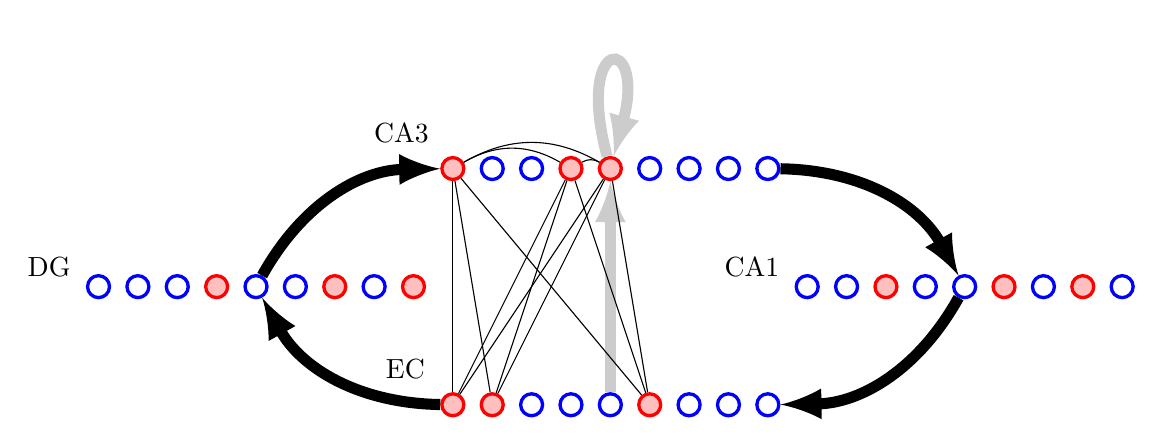
\begin{tikzpicture}
\node[on,text width=0.1cm](EC0){};
\node[on,text width=0.1cm,right of = EC0,xshift = -0.5cm](EC1){};
\node[off,text width=0.1cm,right of = EC1,xshift = -0.5cm](EC2){};
\node[off,text width=0.1cm,right of = EC2,xshift = -0.5cm](EC3){};
\node[off,text width=0.1cm,right of = EC3,xshift = -0.5cm](EC4){};
\node[on,text width=0.1cm,right of = EC4,xshift = -0.5cm](EC5){};
\node[off,text width=0.1cm,right of = EC5,xshift = -0.5cm](EC6){};
\node[off,text width=0.1cm,right of = EC6,xshift = -0.5cm](EC7){};
\node[off,text width=0.1cm,right of = EC7,xshift = -0.5cm](EC8){};

\node[off,text width=0.1cm, left of =EC0, xshift=-3.5cm,yshift=1.5cm](DG0){};
\node[off,text width=0.1cm,right of = DG0,xshift = -0.5cm](DG1){};
\node[off,text width=0.1cm,right of = DG1,xshift = -0.5cm](DG2){};
\node[on,text width=0.1cm,right of = DG2,xshift = -0.5cm](DG3){};
\node[off,text width=0.1cm,right of = DG3,xshift = -0.5cm](DG4){};
\node[off,text width=0.1cm,right of = DG4,xshift = -0.5cm](DG5){};
\node[on,text width=0.1cm,right of = DG5,xshift = -0.5cm](DG6){};
\node[off,text width=0.1cm,right of = DG6,xshift = -0.5cm](DG7){};
\node[on,text width=0.1cm,right of = DG7,xshift = -0.5cm](DG8){};

\node[off,text width=0.1cm, right of =EC8, xshift=-.5cm,yshift=1.5cm](CA10){};
\node[off,text width=0.1cm,right of = CA10,xshift = -0.5cm](CA11){};
\node[on,text width=0.1cm,right of = CA11,xshift = -0.5cm](CA12){};
\node[off,text width=0.1cm,right of = CA12,xshift = -0.5cm](CA13){};
\node[off,text width=0.1cm,right of = CA13,xshift = -0.5cm](CA14){};
\node[on,text width=0.1cm,right of = CA14,xshift = -0.5cm](CA15){};
\node[off,text width=0.1cm,right of = CA15,xshift = -0.5cm](CA16){};
\node[on,text width=0.1cm,right of = CA16,xshift = -0.5cm](CA17){};
\node[off,text width=0.1cm,right of = CA17,xshift = -0.5cm](CA18){};

\node[on,text width=0.1cm, above of =EC0,yshift=2cm](CA30){};
\node[off,text width=0.1cm,right of = CA30,xshift = -0.5cm](CA31){};
\node[off,text width=0.1cm,right of = CA31,xshift = -0.5cm](CA32){};
\node[on,text width=0.1cm,right of = CA32,xshift = -0.5cm](CA33){};
\node[on,text width=0.1cm,right of = CA33,xshift = -0.5cm](CA34){};
\node[off,text width=0.1cm,right of = CA34,xshift = -0.5cm](CA35){};
\node[off,text width=0.1cm,right of = CA35,xshift = -0.5cm](CA36){};
\node[off,text width=0.1cm,right of = CA36,xshift = -0.5cm](CA37){};
\node[off,text width=0.1cm,right of = CA37,xshift = -0.5cm](CA38){};

\draw[->, >=latex, black!20!white, line width=4pt]   (EC4) to (CA34) ;
\draw[->, >=latex, black, line width=4pt, bend left]   (EC0) to (DG4) ;
\draw[->, >=latex, black, line width=4pt, bend left]   (DG4) to (CA30) ;
\draw[->, >=latex, black, line width=4pt, bend left]   (CA38) to (CA14) ;
\draw[->, >=latex, black, line width=4pt, bend left]   (CA14) to (EC8) ;
\draw[->, >=latex, black!20!white, line width=4pt, loop above, looseness=50]   (CA34) to (CA34) ;
\node[inner sep=0,anchor=east,text width=3.3cm, left of = DG0, xshift=1.75cm,yshift=0.25cm] (DGlabel) {DG};
\node[inner sep=0,anchor=east,text width=3.3cm, left of = CA10, xshift=1.6cm,yshift=0.25cm] (DGlabel) {CA1};
\node[inner sep=0,anchor=east,text width=3.3cm, left of = CA30, xshift=1.65cm,yshift=0.45cm] (DGlabel) {CA3};
\node[inner sep=0,anchor=east,text width=3.3cm, left of = EC0, xshift=1.8cm,yshift=0.45cm] (DGlabel) {EC};
\path 
(EC0) edge (CA30)
(EC0) edge (CA33)
(EC0) edge (CA34)
(EC1) edge (CA30)
(EC1) edge (CA33)
(EC1) edge (CA34)
(EC5) edge (CA30)
(EC5) edge (CA33)
(EC5) edge (CA34)
(CA30) edge [bend left] (CA33)
(CA30) edge [bend left] (CA34)
(CA33) edge [bend left] (CA34)
;
\end{tikzpicture}
\end{center}

Now, during retrieval, part of the pattern is presented to EC.
\begin{center}
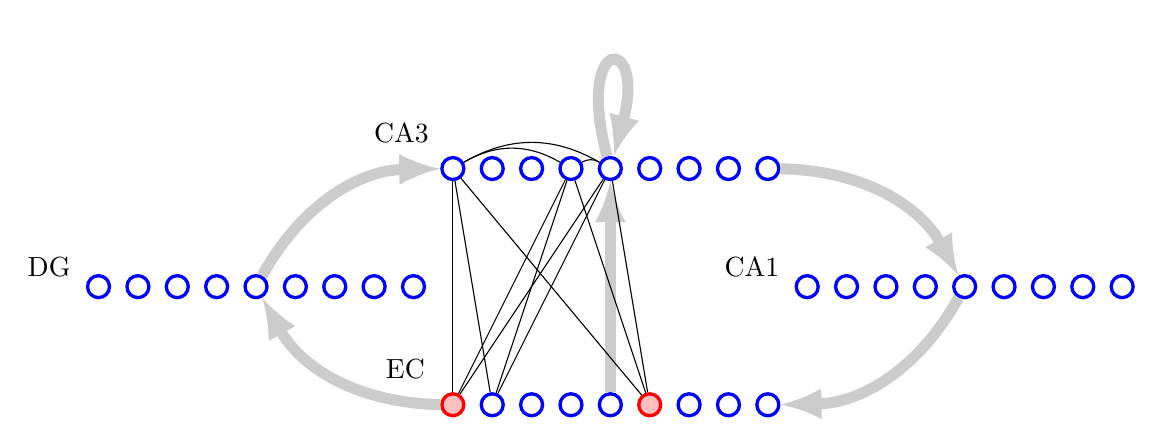
\begin{tikzpicture}
\node[on,text width=0.1cm](EC0){};
\node[off,text width=0.1cm,right of = EC0,xshift = -0.5cm](EC1){};
\node[off,text width=0.1cm,right of = EC1,xshift = -0.5cm](EC2){};
\node[off,text width=0.1cm,right of = EC2,xshift = -0.5cm](EC3){};
\node[off,text width=0.1cm,right of = EC3,xshift = -0.5cm](EC4){};
\node[on,text width=0.1cm,right of = EC4,xshift = -0.5cm](EC5){};
\node[off,text width=0.1cm,right of = EC5,xshift = -0.5cm](EC6){};
\node[off,text width=0.1cm,right of = EC6,xshift = -0.5cm](EC7){};
\node[off,text width=0.1cm,right of = EC7,xshift = -0.5cm](EC8){};

\node[off,text width=0.1cm, left of =EC0, xshift=-3.5cm,yshift=1.5cm](DG0){};
\node[off,text width=0.1cm,right of = DG0,xshift = -0.5cm](DG1){};
\node[off,text width=0.1cm,right of = DG1,xshift = -0.5cm](DG2){};
\node[off,text width=0.1cm,right of = DG2,xshift = -0.5cm](DG3){};
\node[off,text width=0.1cm,right of = DG3,xshift = -0.5cm](DG4){};
\node[off,text width=0.1cm,right of = DG4,xshift = -0.5cm](DG5){};
\node[off,text width=0.1cm,right of = DG5,xshift = -0.5cm](DG6){};
\node[off,text width=0.1cm,right of = DG6,xshift = -0.5cm](DG7){};
\node[off,text width=0.1cm,right of = DG7,xshift = -0.5cm](DG8){};

\node[off,text width=0.1cm, right of =EC8, xshift=-.5cm,yshift=1.5cm](CA10){};
\node[off,text width=0.1cm,right of = CA10,xshift = -0.5cm](CA11){};
\node[off,text width=0.1cm,right of = CA11,xshift = -0.5cm](CA12){};
\node[off,text width=0.1cm,right of = CA12,xshift = -0.5cm](CA13){};
\node[off,text width=0.1cm,right of = CA13,xshift = -0.5cm](CA14){};
\node[off,text width=0.1cm,right of = CA14,xshift = -0.5cm](CA15){};
\node[off,text width=0.1cm,right of = CA15,xshift = -0.5cm](CA16){};
\node[off,text width=0.1cm,right of = CA16,xshift = -0.5cm](CA17){};
\node[off,text width=0.1cm,right of = CA17,xshift = -0.5cm](CA18){};

\node[off,text width=0.1cm, above of =EC0,yshift=2cm](CA30){};
\node[off,text width=0.1cm,right of = CA30,xshift = -0.5cm](CA31){};
\node[off,text width=0.1cm,right of = CA31,xshift = -0.5cm](CA32){};
\node[off,text width=0.1cm,right of = CA32,xshift = -0.5cm](CA33){};
\node[off,text width=0.1cm,right of = CA33,xshift = -0.5cm](CA34){};
\node[off,text width=0.1cm,right of = CA34,xshift = -0.5cm](CA35){};
\node[off,text width=0.1cm,right of = CA35,xshift = -0.5cm](CA36){};
\node[off,text width=0.1cm,right of = CA36,xshift = -0.5cm](CA37){};
\node[off,text width=0.1cm,right of = CA37,xshift = -0.5cm](CA38){};

\draw[->, >=latex, black!20!white, line width=4pt]   (EC4) to (CA34) ;
\draw[->, >=latex, black!20!white, line width=4pt, bend left]   (EC0) to (DG4) ;
\draw[->, >=latex, black!20!white, line width=4pt, bend left]   (DG4) to (CA30) ;
\draw[->, >=latex, black!20!white, line width=4pt, bend left]   (CA38) to (CA14) ;
\draw[->, >=latex, black!20!white, line width=4pt, bend left]   (CA14) to (EC8) ;
\draw[->, >=latex, black!20!white, line width=4pt, loop above, looseness=50]   (CA34) to (CA34) ;
\node[inner sep=0,anchor=east,text width=3.3cm, left of = DG0, xshift=1.75cm,yshift=0.25cm] (DGlabel) {DG};
\node[inner sep=0,anchor=east,text width=3.3cm, left of = CA10, xshift=1.6cm,yshift=0.25cm] (DGlabel) {CA1};
\node[inner sep=0,anchor=east,text width=3.3cm, left of = CA30, xshift=1.65cm,yshift=0.45cm] (DGlabel) {CA3};
\node[inner sep=0,anchor=east,text width=3.3cm, left of = EC0, xshift=1.8cm,yshift=0.45cm] (DGlabel) {EC};
\path 
(EC0) edge (CA30)
(EC0) edge (CA33)
(EC0) edge (CA34)
(EC1) edge (CA30)
(EC1) edge (CA33)
(EC1) edge (CA34)
(EC5) edge (CA30)
(EC5) edge (CA33)
(EC5) edge (CA34)
(CA30) edge [bend left] (CA33)
(CA30) edge [bend left] (CA34)
(CA33) edge [bend left] (CA34)
;
\end{tikzpicture}
\end{center}
Because of the connections from EC to CA3 and the recurrent connections in CA3, this excites the pattern in CA3:
\begin{center}
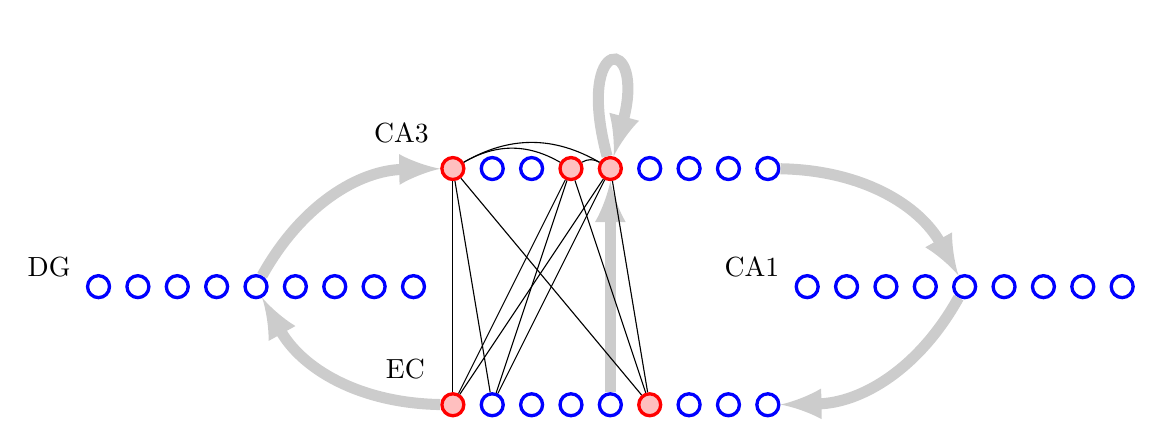
\begin{tikzpicture}
\node[on,text width=0.1cm](EC0){};
\node[off,text width=0.1cm,right of = EC0,xshift = -0.5cm](EC1){};
\node[off,text width=0.1cm,right of = EC1,xshift = -0.5cm](EC2){};
\node[off,text width=0.1cm,right of = EC2,xshift = -0.5cm](EC3){};
\node[off,text width=0.1cm,right of = EC3,xshift = -0.5cm](EC4){};
\node[on,text width=0.1cm,right of = EC4,xshift = -0.5cm](EC5){};
\node[off,text width=0.1cm,right of = EC5,xshift = -0.5cm](EC6){};
\node[off,text width=0.1cm,right of = EC6,xshift = -0.5cm](EC7){};
\node[off,text width=0.1cm,right of = EC7,xshift = -0.5cm](EC8){};

\node[off,text width=0.1cm, left of =EC0, xshift=-3.5cm,yshift=1.5cm](DG0){};
\node[off,text width=0.1cm,right of = DG0,xshift = -0.5cm](DG1){};
\node[off,text width=0.1cm,right of = DG1,xshift = -0.5cm](DG2){};
\node[off,text width=0.1cm,right of = DG2,xshift = -0.5cm](DG3){};
\node[off,text width=0.1cm,right of = DG3,xshift = -0.5cm](DG4){};
\node[off,text width=0.1cm,right of = DG4,xshift = -0.5cm](DG5){};
\node[off,text width=0.1cm,right of = DG5,xshift = -0.5cm](DG6){};
\node[off,text width=0.1cm,right of = DG6,xshift = -0.5cm](DG7){};
\node[off,text width=0.1cm,right of = DG7,xshift = -0.5cm](DG8){};

\node[off,text width=0.1cm, right of =EC8, xshift=-.5cm,yshift=1.5cm](CA10){};
\node[off,text width=0.1cm,right of = CA10,xshift = -0.5cm](CA11){};
\node[off,text width=0.1cm,right of = CA11,xshift = -0.5cm](CA12){};
\node[off,text width=0.1cm,right of = CA12,xshift = -0.5cm](CA13){};
\node[off,text width=0.1cm,right of = CA13,xshift = -0.5cm](CA14){};
\node[off,text width=0.1cm,right of = CA14,xshift = -0.5cm](CA15){};
\node[off,text width=0.1cm,right of = CA15,xshift = -0.5cm](CA16){};
\node[off,text width=0.1cm,right of = CA16,xshift = -0.5cm](CA17){};
\node[off,text width=0.1cm,right of = CA17,xshift = -0.5cm](CA18){};

\node[on,text width=0.1cm, above of =EC0,yshift=2cm](CA30){};
\node[off,text width=0.1cm,right of = CA30,xshift = -0.5cm](CA31){};
\node[off,text width=0.1cm,right of = CA31,xshift = -0.5cm](CA32){};
\node[on,text width=0.1cm,right of = CA32,xshift = -0.5cm](CA33){};
\node[on,text width=0.1cm,right of = CA33,xshift = -0.5cm](CA34){};
\node[off,text width=0.1cm,right of = CA34,xshift = -0.5cm](CA35){};
\node[off,text width=0.1cm,right of = CA35,xshift = -0.5cm](CA36){};
\node[off,text width=0.1cm,right of = CA36,xshift = -0.5cm](CA37){};
\node[off,text width=0.1cm,right of = CA37,xshift = -0.5cm](CA38){};

\draw[->, >=latex, black!20!white, line width=4pt]   (EC4) to (CA34) ;
\draw[->, >=latex, black!20!white, line width=4pt, bend left]   (EC0) to (DG4) ;
\draw[->, >=latex, black!20!white, line width=4pt, bend left]   (DG4) to (CA30) ;
\draw[->, >=latex, black!20!white, line width=4pt, bend left]   (CA38) to (CA14) ;
\draw[->, >=latex, black!20!white, line width=4pt, bend left]   (CA14) to (EC8) ;
\draw[->, >=latex, black!20!white, line width=4pt, loop above, looseness=50]   (CA34) to (CA34) ;
\node[inner sep=0,anchor=east,text width=3.3cm, left of = DG0, xshift=1.75cm,yshift=0.25cm] (DGlabel) {DG};
\node[inner sep=0,anchor=east,text width=3.3cm, left of = CA10, xshift=1.6cm,yshift=0.25cm] (DGlabel) {CA1};
\node[inner sep=0,anchor=east,text width=3.3cm, left of = CA30, xshift=1.65cm,yshift=0.45cm] (DGlabel) {CA3};
\node[inner sep=0,anchor=east,text width=3.3cm, left of = EC0, xshift=1.8cm,yshift=0.45cm] (DGlabel) {EC};
\path 
(EC0) edge (CA30)
(EC0) edge (CA33)
(EC0) edge (CA34)
(EC1) edge (CA30)
(EC1) edge (CA33)
(EC1) edge (CA34)
(EC5) edge (CA30)
(EC5) edge (CA33)
(EC5) edge (CA34)
(CA30) edge [bend left] (CA33)
(CA30) edge [bend left] (CA34)
(CA33) edge [bend left] (CA34)
;
\end{tikzpicture}
\end{center}
This memory is sent back to EC via CA1, and recall has occurred!
\begin{center}
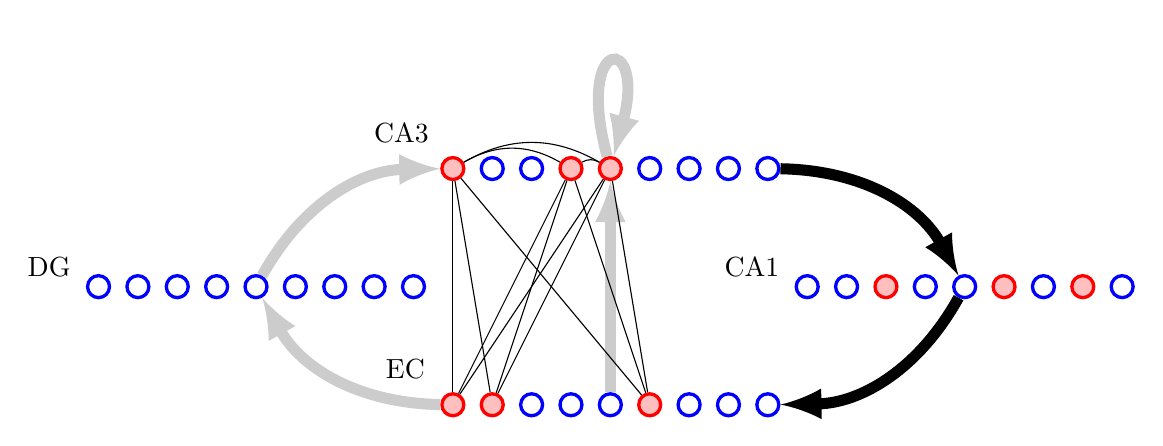
\begin{tikzpicture}
\node[on,text width=0.1cm](EC0){};
\node[on,text width=0.1cm,right of = EC0,xshift = -0.5cm](EC1){};
\node[off,text width=0.1cm,right of = EC1,xshift = -0.5cm](EC2){};
\node[off,text width=0.1cm,right of = EC2,xshift = -0.5cm](EC3){};
\node[off,text width=0.1cm,right of = EC3,xshift = -0.5cm](EC4){};
\node[on,text width=0.1cm,right of = EC4,xshift = -0.5cm](EC5){};
\node[off,text width=0.1cm,right of = EC5,xshift = -0.5cm](EC6){};
\node[off,text width=0.1cm,right of = EC6,xshift = -0.5cm](EC7){};
\node[off,text width=0.1cm,right of = EC7,xshift = -0.5cm](EC8){};

\node[off,text width=0.1cm, left of =EC0, xshift=-3.5cm,yshift=1.5cm](DG0){};
\node[off,text width=0.1cm,right of = DG0,xshift = -0.5cm](DG1){};
\node[off,text width=0.1cm,right of = DG1,xshift = -0.5cm](DG2){};
\node[off,text width=0.1cm,right of = DG2,xshift = -0.5cm](DG3){};
\node[off,text width=0.1cm,right of = DG3,xshift = -0.5cm](DG4){};
\node[off,text width=0.1cm,right of = DG4,xshift = -0.5cm](DG5){};
\node[off,text width=0.1cm,right of = DG5,xshift = -0.5cm](DG6){};
\node[off,text width=0.1cm,right of = DG6,xshift = -0.5cm](DG7){};
\node[off,text width=0.1cm,right of = DG7,xshift = -0.5cm](DG8){};


\node[off,text width=0.1cm, right of =EC8, xshift=-.5cm,yshift=1.5cm](CA10){};
\node[off,text width=0.1cm,right of = CA10,xshift = -0.5cm](CA11){};
\node[on,text width=0.1cm,right of = CA11,xshift = -0.5cm](CA12){};
\node[off,text width=0.1cm,right of = CA12,xshift = -0.5cm](CA13){};
\node[off,text width=0.1cm,right of = CA13,xshift = -0.5cm](CA14){};
\node[on,text width=0.1cm,right of = CA14,xshift = -0.5cm](CA15){};
\node[off,text width=0.1cm,right of = CA15,xshift = -0.5cm](CA16){};
\node[on,text width=0.1cm,right of = CA16,xshift = -0.5cm](CA17){};
\node[off,text width=0.1cm,right of = CA17,xshift = -0.5cm](CA18){};

\node[on,text width=0.1cm, above of =EC0,yshift=2cm](CA30){};
\node[off,text width=0.1cm,right of = CA30,xshift = -0.5cm](CA31){};
\node[off,text width=0.1cm,right of = CA31,xshift = -0.5cm](CA32){};
\node[on,text width=0.1cm,right of = CA32,xshift = -0.5cm](CA33){};
\node[on,text width=0.1cm,right of = CA33,xshift = -0.5cm](CA34){};
\node[off,text width=0.1cm,right of = CA34,xshift = -0.5cm](CA35){};
\node[off,text width=0.1cm,right of = CA35,xshift = -0.5cm](CA36){};
\node[off,text width=0.1cm,right of = CA36,xshift = -0.5cm](CA37){};
\node[off,text width=0.1cm,right of = CA37,xshift = -0.5cm](CA38){};

\draw[->, >=latex, black!20!white, line width=4pt]   (EC4) to (CA34) ;
\draw[->, >=latex, black!20!white, line width=4pt, bend left]   (EC0) to (DG4) ;
\draw[->, >=latex, black!20!white, line width=4pt, bend left]   (DG4) to (CA30) ;
\draw[->, >=latex, black, line width=4pt, bend left]   (CA38) to (CA14) ;
\draw[->, >=latex, black, line width=4pt, bend left]   (CA14) to (EC8) ;
\draw[->, >=latex, black!20!white, line width=4pt, loop above, looseness=50]   (CA34) to (CA34) ;
\node[inner sep=0,anchor=east,text width=3.3cm, left of = DG0, xshift=1.75cm,yshift=0.25cm] (DGlabel) {DG};
\node[inner sep=0,anchor=east,text width=3.3cm, left of = CA10, xshift=1.6cm,yshift=0.25cm] (DGlabel) {CA1};
\node[inner sep=0,anchor=east,text width=3.3cm, left of = CA30, xshift=1.65cm,yshift=0.45cm] (DGlabel) {CA3};
\node[inner sep=0,anchor=east,text width=3.3cm, left of = EC0, xshift=1.8cm,yshift=0.45cm] (DGlabel) {EC};
\path 
(EC0) edge (CA30)
(EC0) edge (CA33)
(EC0) edge (CA34)
(EC1) edge (CA30)
(EC1) edge (CA33)
(EC1) edge (CA34)
(EC5) edge (CA30)
(EC5) edge (CA33)
(EC5) edge (CA34)
(CA30) edge [bend left] (CA33)
(CA30) edge [bend left] (CA34)
(CA33) edge [bend left] (CA34)
;
\end{tikzpicture}
\end{center}

This doesn't explain how the hippocampus switches between the learning
and retrieval phase. One suggestion is just that the level of stimulus
is different, that larger activity during learning excites the pathway that goes via DG \cite{OReillyMcClelland1994a}, another is that the neuromodulator acetylcholine \cite{Hasselmo2006a} or dopamine \cite{LismanGrace2005a} is important.


\begin{thebibliography}{10}

\bibitem{OKeefeDostrovsky1971a}
O'Keefe J, Dostrovsky J. (1971) The hippocampus as a spatial map. Preliminary evidence from unit activity in the freely-moving rat.
\newblock Brain Research 34: 171--5.

\bibitem{QuianQuirogalEtAl2005a}
Quian Quiroga R, Reddy L, Kreiman G, Koch C, Fried I. (2005) Invariant visual representation by single neurons in the human brain.
\newblock Nature 435: 1102--7.

\bibitem{McCullochPitts1943a}
McCulloch W, Pitts W. (1943). A logical calculus of the ideas immanent in nervous activity. 
\newblock Bulletin of Mathematical Biophysics 7: 115--33.

\bibitem{Amit1992a} Amit D. (1992) Modeling Brain Function: The World
  of Attractor Neural Networks.
\newblock Cambridge University Press, Cambridge England.

\bibitem{OReillyMunakata2000a}
O'Reilly RC, Munakata Y (2000) Computational explorations in cognitive neuroscience: Understanding the mind by simulating the brain.
\newblock MIT press, Cambridge MA.

\bibitem{OReillyMcClelland1994a}
O’Reilly RC, McClelland JL (1994) Hippocampal conjunctive encoding, storage, and recall: Avoiding a tradeoff.
\newblock Hippocampus 4: 661--82.

\bibitem{Hasselmo2006a}
Hasselmo ME. (2006) The role of acetylcholine in learning and memory.
\newblock Current Opinion in Neurobiology 16: 710--71

\bibitem{LismanGrace2005a}
Lisman JE, Grace AA. (2005) The hippocampal-VTA loop: controlling the entry of information into long-term memory.
\newblock Neuron, 46: 703--713.

\end{thebibliography}

\end{document}
